%% =============================================================
%%  Les valeurs — de la ronde aux groupes irréguliers
%%  Guide de référence, composé en LaTeX, gravures LilyPond
%% =============================================================
%%
%%  Les figures (gravures/v-*.cropped.pdf), le tableau des figures
%%  (gravures/valeurs-tableau.tex), les exercices et leurs réponses
%%  (gravures/valeurs-questions.tex, gravures/valeurs-reponses.tex) et
%%  le fichier valeurs.musicxml sont produits par
%%  outils/generer_valeurs.py. Voir le colophon en dernière page.
%%
\documentclass[a4paper,11pt]{article}

\usepackage[top=2.2cm,bottom=2.4cm,left=2.2cm,right=2.2cm]{geometry}
\usepackage[T1]{fontenc}
\usepackage[utf8]{inputenc}
\usepackage[french]{babel}
\usepackage{lmodern}
\usepackage{xcolor}
\usepackage{graphicx}
\usepackage{titlesec}
\usepackage{fancyhdr}
\usepackage{mdframed}
\usepackage{enumitem}
\usepackage{booktabs}
\usepackage{multicol}
\usepackage{hyperref}

\graphicspath{{gravures/}}

% ---- Couleurs, reprises du document des accords de guitare ---------
\definecolor{navy}{RGB}{18,50,105}
\definecolor{lightnavy}{RGB}{235,241,255}
\definecolor{mygray}{RGB}{110,110,110}

\hypersetup{colorlinks=true, linkcolor=navy, urlcolor=navy,
  pdftitle={Les valeurs — de la ronde aux groupes irréguliers},
  pdfauthor={Fabian Bastin}}

% ---- En-tête et pied -----------------------------------------------
\pagestyle{fancy}
\fancyhf{}
\renewcommand{\headrulewidth}{0.4pt}
\renewcommand{\footrulewidth}{0.4pt}
\fancyhead[L]{\small\bfseries\textcolor{navy}{Les valeurs}}
\fancyhead[R]{\small\textcolor{mygray}{\thepage}}
\fancyfoot[C]{\small\textcolor{mygray}{De la ronde aux groupes irréguliers}}

% ---- Titres de section ---------------------------------------------
\newcommand{\navysect}[1]{%
  \colorbox{navy}{%
    \parbox[c][17pt]{\dimexpr\linewidth-2\fboxsep\relax}{%
      \color{white}\hspace{6pt}\bfseries\normalsize #1}}%
}
\titleformat{\section}[block]{\normalfont}{}{0pt}{\navysect}
\titlespacing*{\section}{0pt}{16pt}{10pt}

% ---- Encadré de remarque -------------------------------------------
\newmdenv[linecolor=navy, linewidth=0.5pt, backgroundcolor=lightnavy,
  innertopmargin=6pt, innerbottommargin=6pt,
  innerleftmargin=8pt, innerrightmargin=8pt,
  skipabove=8pt, skipbelow=8pt]{remarque}

% ---- Figure gravée ---------------------------------------------------
% Figure gravée, à la largeur donnée (part de la ligne), avec sa légende.
% Le tout tient dans une minipage : figure et légende ne sont jamais
% séparées par un saut de page. Les largeurs sont proportionnelles aux
% largeurs naturelles des gravures : toutes sont à la même échelle.
\newcommand{\gravure}[3]{%
  \par\medskip\noindent
  \begin{minipage}{\linewidth}
    \centering
    \includegraphics[width=#2\linewidth]{#1.cropped.pdf}\\[4pt]
    {\small\itshape\color{mygray} #3}
  \end{minipage}\par\medskip
}

% Légende seule, sous un tableau.
\newcommand{\legende}[1]{\\[4pt]{\small\itshape\color{mygray} #1}}

\setlist{itemsep=2pt, topsep=4pt, parsep=0pt}

\begin{document}

% =====================================================================
\begin{titlepage}
\centering
\vspace*{3cm}
{\Huge\bfseries\color{navy} Les valeurs\par}
\vspace{0.6cm}
{\LARGE\color{navy} De la ronde aux groupes irréguliers\par}
\vspace{1.4cm}
{\large Une ronde, deux blanches, quatre noires\par}
\vspace{2.5cm}
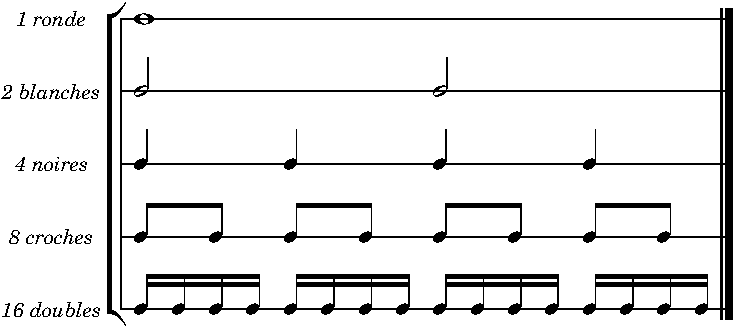
\includegraphics[width=0.71\linewidth]{v-arbre.cropped.pdf}
\vfill
{\small\color{mygray}
Gravures LilyPond, composition \LaTeX.\\
Fichier MusicXML joint.\par}
\vspace{1cm}
\end{titlepage}

\tableofcontents
\newpage

% =====================================================================
\section{Avant-propos}

La \textbf{valeur} d'une note est sa durée, lue sur sa figure : une blanche
dure deux noires, une noire deux croches. Cette durée est relative. Ce que
dure une noire en secondes, c'est le mouvement qui le fixe ; la figure dit
seulement le rapport de sa durée à celle des autres.

À lire après
\href{https://www.slashbin.net/musique/theorie/lecture.pdf}{\emph{Lire les
notes}}, pour la portée et la clé de sol. \href{https://www.slashbin.net/musique/theorie/mesure.pdf}{\emph{La mesure}} range ensuite ces
valeurs en temps et en mesures. Au programme de matières théoriques de l'École
de musique Vincent-d'Indy, ces notions relèvent des niveaux 1 à 4.

\begin{remarque}
\textbf{Conventions.} Les exemples sont en clé de sol, sans chiffres
indicateurs : il s'agit ici de durées, non de mesures. La plupart sont écrits
sur la3, le la du diapason, au deuxième interligne. Les barres séparent les
exemples. Les durées en secondes supposent le mouvement du fichier MusicXML,
la noire à 60 : une noire par seconde.
\end{remarque}

Le fichier MusicXML joint fait entendre chaque exemple ; la
section~\ref{sec:musicxml} le présente.

% =====================================================================
\section{Les figures de notes}
\label{sec:figures}

\textbf{Trois éléments.} Une figure de note se compose d'une \emph{tête},
ovale, blanche (évidée) ou noire (pleine) ; d'une \emph{hampe}, trait vertical
attaché à la tête ; et de \emph{crochets}, au bout de la hampe. La ronde n'a
que sa tête ; la blanche y ajoute une hampe ; la noire noircit la tête ; la
croche porte un crochet, et chaque figure suivante un crochet de plus.

\gravure{v-notes}{0.78}{Les sept figures de notes usuelles, de la plus longue à la plus
brève.}

\textbf{Le sens de la hampe.} Au-dessous de la troisième ligne, la hampe monte,
à droite de la tête ; au-dessus, elle descend, à gauche. Sur la troisième
ligne, elle descend le plus souvent. Le crochet, lui, part toujours vers la
droite.

\textbf{La ligature.} Plusieurs croches, ou valeurs plus brèves, se réunissent
par une \emph{ligature}, une barre épaisse qui remplace leurs crochets : une
barre par crochet, deux pour les doubles croches, trois pour les triples. On
ligature d'ordinaire les notes d'un même temps, ce que traite \emph{La mesure}.

\gravure{v-anatomie}{0.48}{Une croche à hampe montante, une croche à hampe
descendante, deux croches réunies par une ligature.}

% =====================================================================
\section{Les silences}
\label{sec:silences}

À chaque figure de note répond un \textbf{silence} de même valeur : la
musique s'arrête, mais le temps continue de s'écouler. La pause vaut une
ronde, la demi-pause une blanche, le soupir une noire ; le demi-soupir, une
croche, porte un crochet, et chaque silence plus bref un crochet de plus.

\gravure{v-silences}{0.88}{Les sept silences, dans l'ordre des figures de
notes.}

\textbf{La pause et la demi-pause.} Les deux sont un petit rectangle plein ; seule
la place les distingue. La pause pend sous la quatrième ligne, la demi-pause
est posée sur la troisième. La pause sert aussi à noter une mesure entière de
silence, quels qu'en soient les chiffres indicateurs.

\textbf{La carrée et le bâton de pause.} Plus longue que la ronde, la
\emph{carrée}, ou brève, vaut deux rondes ; son silence, le \emph{bâton de
pause}, remplit l'interligne qui le porte. On ne les rencontre plus guère que
dans la musique ancienne et dans les mesures à 4/2.

\textbf{Les mesures à compter.} Une longue suite de mesures de silence ne
s'écrit pas pause après pause : un trait épais posé sur la troisième ligne,
surmonté du nombre de mesures, les réunit. Le musicien les compte en attendant
d'entrer ; les parties d'orchestre en sont pleines.

\gravure{v-longues}{0.63}{La carrée et le bâton de pause, chacun dans une
mesure à 4/2 ; puis, à 4/4, huit mesures à compter avant que la musique
reprenne.}

% =====================================================================
\section{Les valeurs relatives}
\label{sec:relatives}

\textbf{Chaque figure vaut deux fois la suivante.} Une ronde vaut deux
blanches, une blanche deux noires, une noire deux croches, et ainsi de suite
jusqu'à la quadruple croche. L'arbre des valeurs le montre étage par étage :
chacun dure une ronde et compte deux fois plus de notes que le précédent.

\gravure{v-arbre}{0.71}{L'arbre des valeurs, de la ronde à la double croche.
Les notes d'une même colonne commencent au même instant.}

\begin{center}
%% Produit par outils/generer_valeurs.py — ne pas modifier à la main.

\begin{tabular}{@{}l l c r r@{}}
\toprule
\textbf{Note} & \textbf{Silence} & \textbf{Crochets} & \textbf{Dans une ronde} & \textbf{À la noire 60} \\
\midrule
ronde & pause & -- & 1 & 4~s \\
blanche & demi-pause & -- & 2 & 2~s \\
noire & soupir & -- & 4 & 1~s \\
croche & demi-soupir & 1 & 8 & $\frac{1}{2}$~s \\
double croche & quart de soupir & 2 & 16 & $\frac{1}{4}$~s \\
triple croche & huitième de soupir & 3 & 32 & $\frac{1}{8}$~s \\
quadruple croche & seizième de soupir & 4 & 64 & $\frac{1}{16}$~s \\
\bottomrule
\end{tabular}

\legende{Les figures de notes, leurs silences, et leur valeur : combien en
contient une ronde, combien de secondes elles durent à la noire 60.}
\end{center}

\textbf{La valeur est relative.} Le tableau donne des secondes pour un
mouvement : la noire à 60. Dans un mouvement plus lent, toutes les durées
s'allongent ensemble ; dans un plus vif, toutes raccourcissent. Le rapport entre les figures, lui, ne change
jamais. Les indications de mouvement relèvent de \href{https://www.slashbin.net/musique/theorie/interpretation.pdf}{\emph{L'interprétation}}.

\begin{remarque}
\textbf{Les noms anglais.} Les partitions et les logiciels en anglais comptent
les figures en fractions de ronde : \emph{whole note}, \emph{half note},
\emph{quarter note}, \emph{eighth note}, \emph{sixteenth note},
\emph{thirty-second note}, \emph{sixty-fourth note}. L'anglais britannique
emploie d'autres noms : \emph{semibreve}, \emph{minim}, \emph{crotchet},
\emph{quaver}, \emph{semiquaver}, \emph{demisemiquaver},
\emph{hemidemisemiquaver}.
\end{remarque}

% =====================================================================
\section{Le point d'augmentation}
\label{sec:point}

\textbf{La moitié en plus.} Un point placé à droite de la tête augmente la
note de la moitié de sa valeur. Une blanche pointée vaut une blanche et une
noire, soit trois noires ; une noire pointée, trois croches ; une croche
pointée, trois doubles croches. Le point s'applique de même aux silences : un
soupir pointé vaut un soupir et un demi-soupir.

\textbf{Le double point.} Un second point ajoute la moitié de ce qu'ajoutait
le premier. Une blanche doublement pointée vaut une blanche, une noire et une
croche, soit sept croches. Un troisième point, rare, ajoute encore la moitié du
deuxième ajout : une blanche triplement pointée vaut quinze doubles croches.

\gravure{v-point}{0.94}{En haut, des valeurs pointées ; en bas, la même durée
sans point, en notes liées ou en silences successifs.}

\textbf{Où se place le point.} Quand la tête est sur une ligne, le point
se met dans l'interligne au-dessus, pour rester lisible.

% =====================================================================
\section{La liaison}
\label{sec:liaison}

\textbf{La liaison de prolongation.} Une courbe qui relie deux notes de même
hauteur les fond en une seule : la seconde n'est pas rejouée, et sa valeur
s'ajoute à celle de la première. Elle permet d'écrire les durées qu'aucune
figure ne donne, même pointée : cinq croches s'écrivent par une blanche liée à
une croche. Elle permet aussi de prolonger une note au-delà de la barre de
mesure, ce que le point ne fait jamais.

\textbf{La liaison d'expression.} La même courbe, posée sur des notes de
hauteurs différentes, ne change aucune durée : elle demande de les enchaîner
sans interruption, \emph{legato}. \emph{L'interprétation} en traite avec les
autres articulations.

\gravure{v-liaisons}{0.45}{Une blanche liée à une croche, qui dure cinq
croches ; puis quatre noires sous une liaison d'expression.}

\textbf{Les distinguer.} La liaison de prolongation relie deux têtes de même
hauteur, voisines ; la liaison d'expression embrasse un groupe de notes
différentes, souvent plus de deux.

% =====================================================================
\section{Le point d'orgue}
\label{sec:point-orgue}

Le \textbf{point d'orgue} est un arc surmonté d'un point, au-dessus d'une note
ou d'un silence ; il se place parfois sous la portée, retourné. Sur un
silence, il prend aussi le nom de \emph{point d'arrêt}.
Il suspend la mesure : la note, ou le silence, se prolonge au-delà de sa
valeur, aussi longtemps que l'interprète, ou le chef, le juge bon. Aucune
règle n'en fixe la durée.

\gravure{v-point-orgue}{0.33}{Le point d'orgue sur une note, puis sur un
silence : un point d'arrêt.}

On le trouve en fin de pièce, sur la dernière note, et à la fin d'une section,
avant que la musique reparte. Dans un concerto, il annonce souvent la
\emph{cadence}, passage que le soliste joue seul et librement.

% =====================================================================
\section{Le triolet et le sextolet}
\label{sec:triolet}

Une noire se divise régulièrement en deux croches, une croche en deux doubles :
chaque division coupe la valeur en deux. Le \textbf{groupe irrégulier} la
divise autrement, et un chiffre le signale, au-dessus ou au-dessous des notes,
dans un trait coudé quand aucune ligature ne les réunit.

\textbf{Le triolet.} Trois notes dans le temps de deux de même figure : trois
croches de triolet dans une noire, trois noires dans une blanche, trois
doubles croches dans une croche. Chaque note dure les deux tiers de sa valeur
écrite. Le chiffre est un 3.

\textbf{Le sextolet.} Six notes dans le temps de quatre de même figure : six
doubles croches dans une noire. Le chiffre est un 6.

\gravure{v-triolets}{0.88}{En haut, la division régulière ; en bas, le groupe
irrégulier qui la remplace, dans la même durée.}

\begin{remarque}
\textbf{Le sextolet et le double triolet.} Les traités ne s'accordent pas sur
la manière de grouper les six notes d'un sextolet : les uns l'entendent comme
deux triolets, appuyés sur la première et la quatrième note ; les autres comme
trois groupes de deux. Les ligatures, ou le contexte, tranchent : deux
triolets s'écrivent souvent comme tels, chacun avec son 3.
\end{remarque}

% =====================================================================
\section{Les autres groupes irréguliers}
\label{sec:groupes}

\textbf{Le duolet et le quartolet.} Une noire pointée se divise régulièrement
en trois croches : c'est le temps des mesures composées, que décrit \emph{La
mesure}. Le \emph{duolet} y loge deux croches, le \emph{quartolet} quatre ;
leurs chiffres sont 2 et 4.

\textbf{Le quintolet, le septolet.} Cinq notes, ou sept, dans le temps de
quatre : cinq ou sept doubles croches dans une noire. Le principe vaut pour
tout nombre ; le chiffre donne toujours le nombre de notes du groupe.

\gravure{v-groupes}{0.93}{En haut, la division régulière ; en bas, le duolet
et le quartolet dans une noire pointée, le quintolet et le septolet dans une
noire.}

\textbf{La figure du groupe.} Un groupe irrégulier emprunte la figure de la
division régulière qu'il remplace : croches pour le duolet et le quartolet,
qui remplacent trois croches ; doubles croches pour le quintolet et le
septolet, qui en remplacent quatre.

\begin{remarque}
\textbf{D'autres écritures.} L'usage varie d'un éditeur à l'autre. Le duolet
s'écrit aussi en deux croches pointées, qui remplissent exactement la noire
pointée, sans chiffre. Pour les grands groupes, certains précisent le rapport
en entier, \emph{\NoAutoSpacing 7:4} plutôt que \emph{7}.
\end{remarque}

% =====================================================================
\section{S'exercer}
\label{sec:exercices}

Pour chaque groupe numéroté, donner sa durée en noires.

\gravure{v-exercice}{0.91}{Dix groupes, séparés par des barres.}

Puis compter combien de valeurs brèves remplissent une valeur longue :
combien de

%% Produit par outils/generer_valeurs.py — ne pas modifier à la main.

\begin{multicols}{2}
\raggedright
\begin{enumerate}[label=\alph*)]
  \item doubles croches dans une blanche pointée~;
  \item croches dans une blanche doublement pointée~;
  \item triples croches dans une noire pointée~;
  \item demi-soupirs dans un soupir pointé~;
  \item quadruples croches dans une croche~;
  \item croches de triolet dans une blanche~;
  \item doubles croches de sextolet dans une blanche~;
  \item soupirs dans une pause.
\end{enumerate}
\end{multicols}


\begin{remarque}
\textbf{Réponses.}

%% Produit par outils/generer_valeurs.py — ne pas modifier à la main.
\emph{Groupes.} 1~:~4~noires~; 2~:~3~noires~; 3~:~2~noires~; 4~:~2~noires et demie~; 5~:~3~noires et demie~; 6~:~3~noires~; 7~:~3~noires et demie~; 8~:~2~noires~; 9~:~4~noires~; 10~:~3~noires.

\emph{Questions.} a)~12~; b)~7~; c)~12~; d)~3~; e)~8~; f)~6~; g)~12~; h)~4~; i)~8.

\end{remarque}

% =====================================================================
\section{Le fichier MusicXML}
\label{sec:musicxml}

Le fichier joint, \texttt{valeurs.musicxml}, fait entendre les exemples à la
noire 60 : les figures de la ronde à la quadruple croche, une mesure chacune ;
chaque note pointée suivie de la même durée sans point ; la blanche liée à une
croche, suivie des cinq croches qu'elle vaut ; le point d'orgue ; chaque groupe irrégulier après la division régulière qu'il
remplace. Viennent ensuite les groupes de l'exercice, une mesure chacun : ses
chiffres indicateurs en donnent la durée, à n'ouvrir qu'après avoir répondu.

Le point d'orgue y est noté ; sa durée étant libre, chaque logiciel la règle à
sa façon, et certains jouent simplement la valeur écrite. La liaison
d'expression n'y figure pas : elle change la manière de jouer, non la durée. Le
fichier se lit avec MuseScore, Finale, Sibelius, Dorico ou tout éditeur de
partitions ; sur slashbin.net, il s'écoute aussi dans Sodor Piano.

% =====================================================================
\section*{Colophon}
\addcontentsline{toc}{section}{Colophon}

Les gravures musicales sont produites par \textbf{LilyPond}, la composition
par \textbf{\LaTeX}. Les gravures, le tableau des figures, les exercices,
leurs réponses et le fichier MusicXML dérivent d'un même modèle, le module
\texttt{generer\_valeurs.py} du dossier \texttt{outils} : une valeur y est une
fraction de ronde, et la durée d'un groupe se calcule. Avant d'écrire quoi que
ce soit, le générateur vérifie ce que le texte affirme : chaque figure vaut
deux fois la suivante, le point ajoute la moitié de la valeur, un groupe
irrégulier dure autant que la division régulière qu'il remplace, et les deux
portées de chaque figure comparative durent autant l'une que l'autre. Pour
régénérer l'ensemble :

\begin{center}
\texttt{python3 outils/generer\_valeurs.py}\\
\texttt{(cd gravures \&\& lilypond -dcrop --formats=pdf v-*.ly)}\\
\texttt{pdflatex valeurs.tex}
\end{center}

\end{document}
